% STAN architecture — 3-stream convergence layout + companion panels.
% Style modelled on HDML_Model/.../architecture_tikz.tex (card + dashed lane style).
% Build: xelatex stan_architecture.tex && pdftocairo -svg / -png
\documentclass[border={24pt 18pt 20pt 18pt}, multi, tikz]{standalone}
\usepackage{amsmath}
\usepackage{xcolor}
\usepackage{fontspec}
\IfFontExistsTF{Times New Roman}{
  \setmainfont{Times New Roman}
}{
  \IfFontExistsTF{Tinos}{
    \setmainfont{Tinos}
  }{
    \setmainfont{Liberation Serif}
  }
}
% math font matched to the serif text (Times -> TeX Gyre Termes Math)
\usepackage{unicode-math}
\setmathfont{TeX Gyre Termes Math}
\usetikzlibrary{positioning, fit, backgrounds, calc, arrows.meta, shadows, shapes.geometric}

% ---------------------------------------------------------------- palette
\definecolor{c_in}{HTML}{4F46E5}      % inputs
\definecolor{c_in_bg}{HTML}{EEF2FF}

\definecolor{c_lin}{HTML}{0284C7}     % linear / embedding / projection
\definecolor{c_lin_bg}{HTML}{E0F2FE}

\definecolor{c_mod}{HTML}{7C3AED}     % FiLM / concatenation (modulation)
\definecolor{c_mod_bg}{HTML}{F3E8FF}

\definecolor{c_tmp}{HTML}{D97706}     % temporal + interaction (TCN, attention)
\definecolor{c_tmp_bg}{HTML}{FEF3C7}

\definecolor{c_out}{HTML}{059669}     % output / likelihood
\definecolor{c_out_bg}{HTML}{D1FAE5}

\definecolor{c_arrow}{HTML}{1E293B}
\definecolor{c_muted}{HTML}{64748B}
\definecolor{c_lane}{HTML}{94A3B8}

\begin{document}
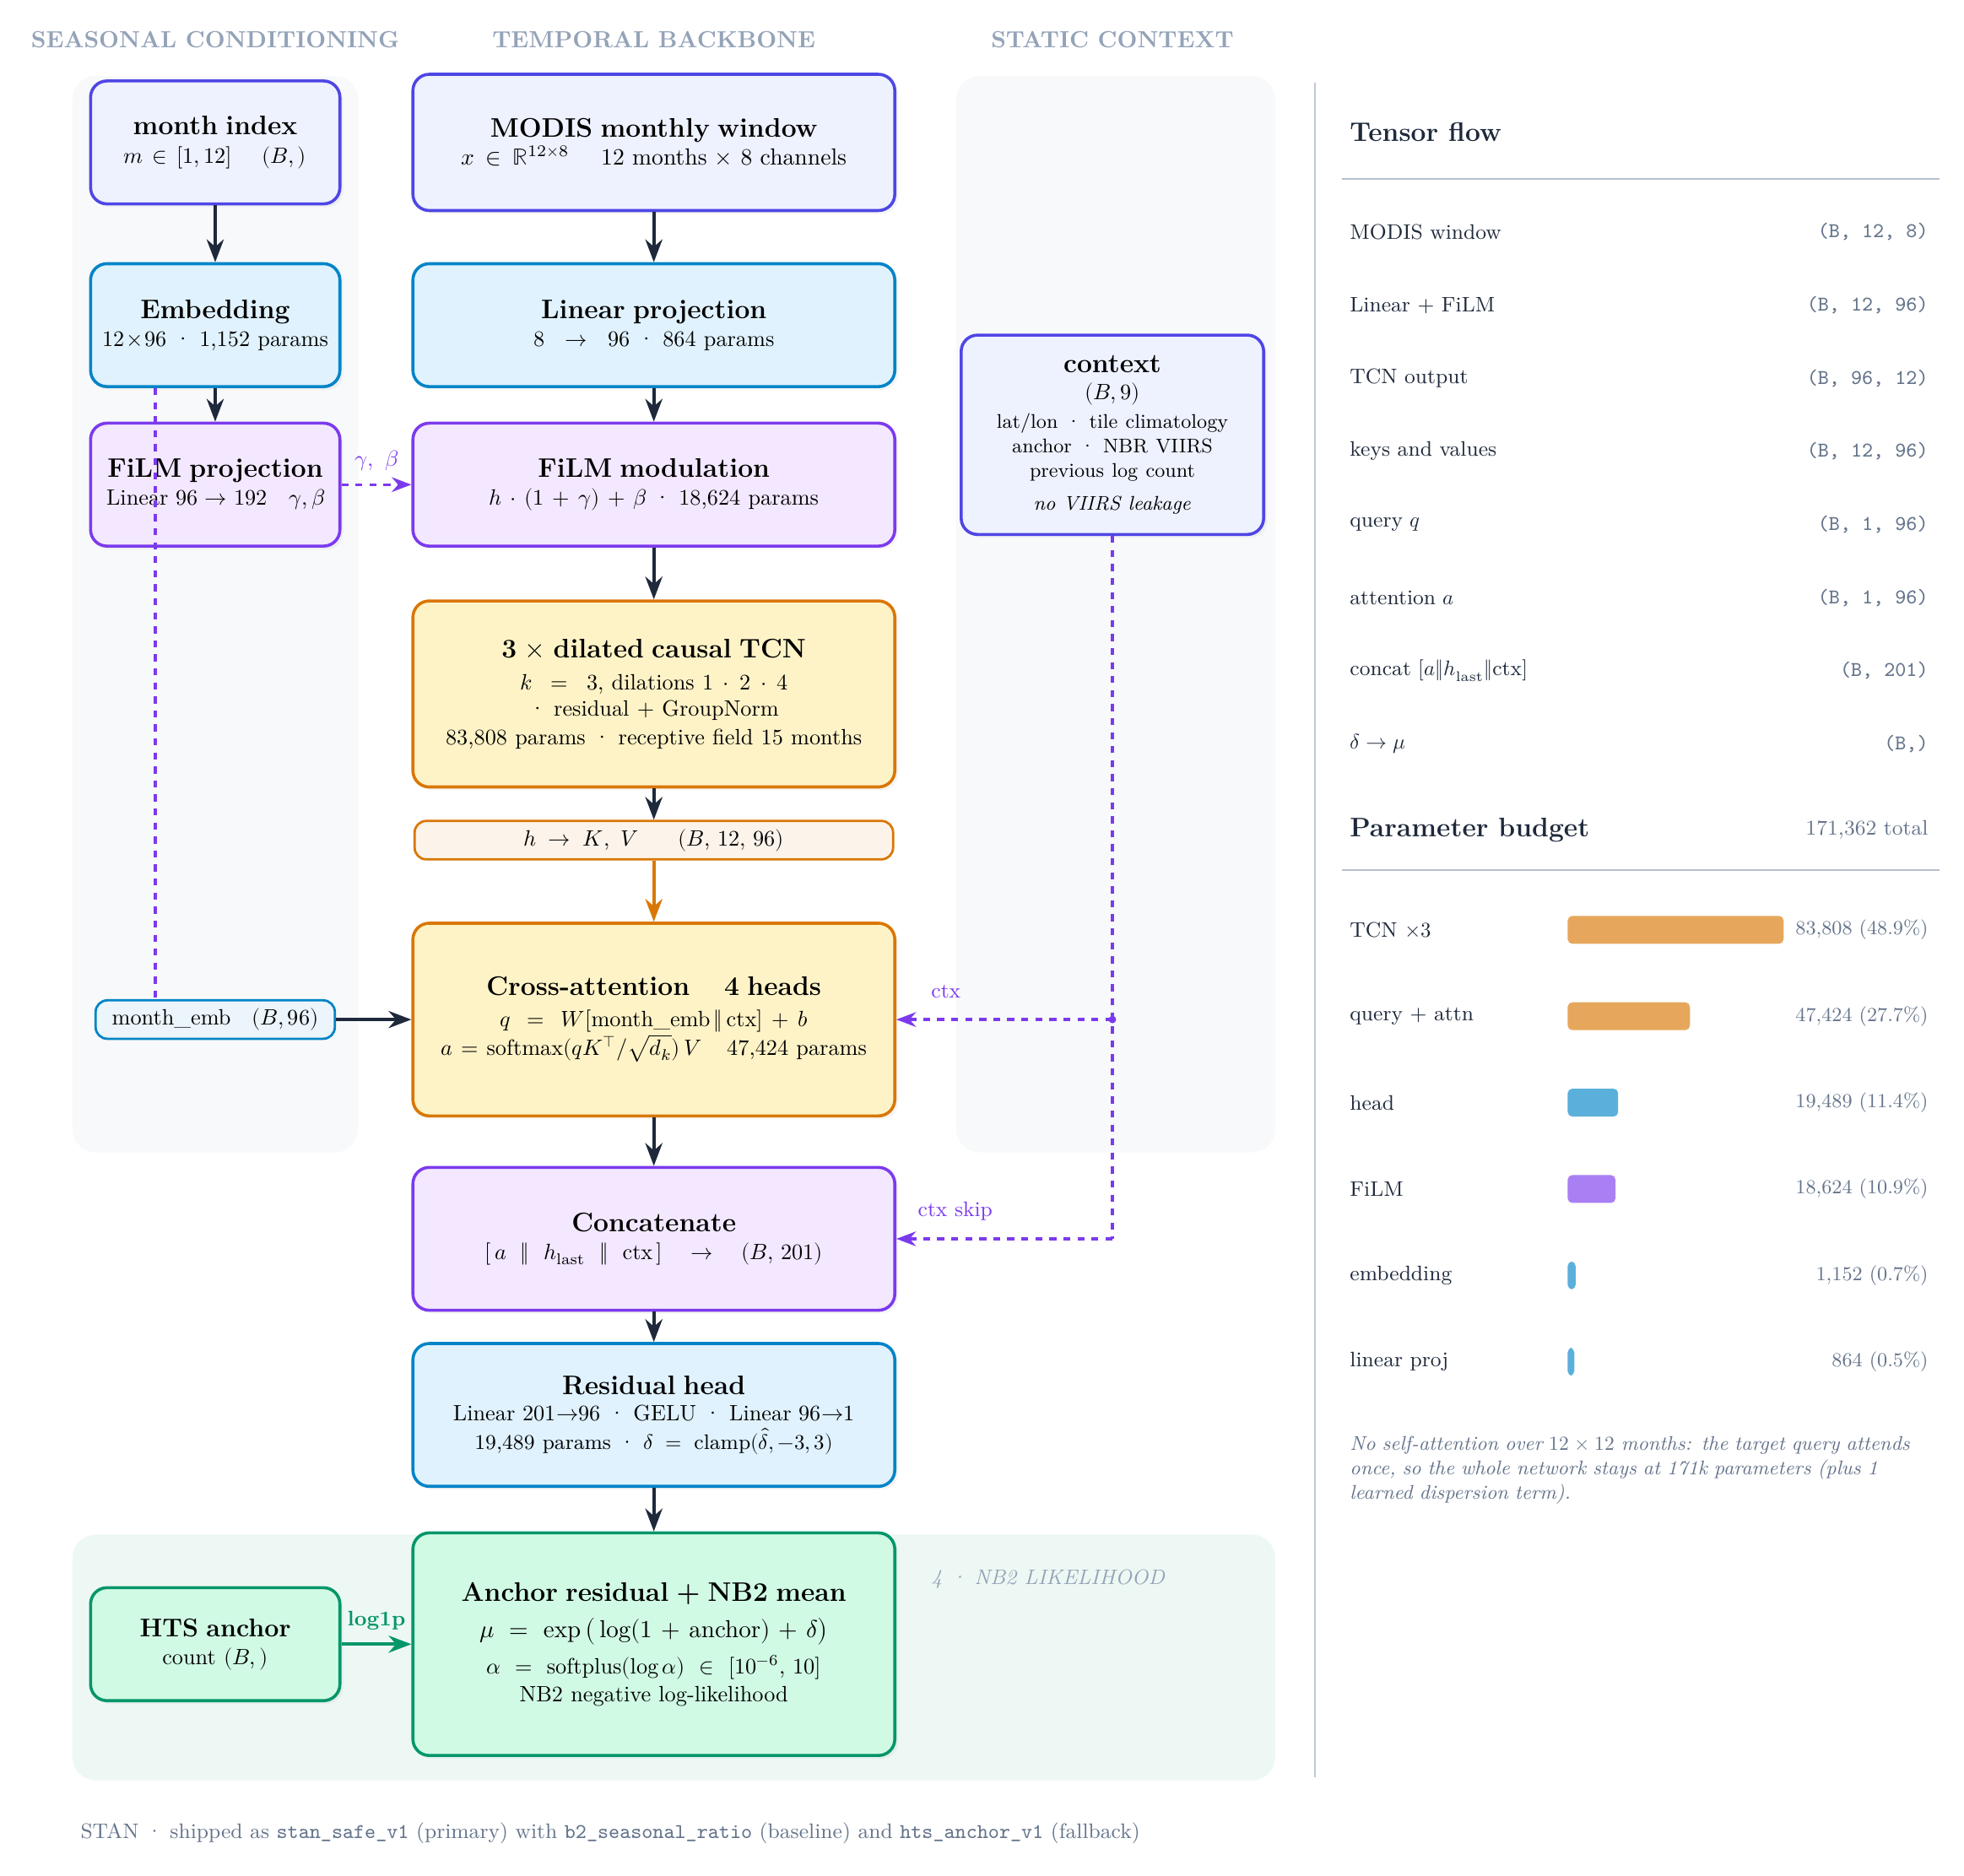
\begin{tikzpicture}[
    >=Stealth,
    card/.style={
        rectangle, rounded corners=7pt, draw=#1, line width=1.3pt,
        fill=white, drop shadow={opacity=0.08, shadow xshift=1.4pt, shadow yshift=-1.4pt},
        align=center, inner sep=5pt
    },
    chip/.style={
        rectangle, rounded corners=5pt, draw=#1, line width=1.0pt, fill=#1!8,
        align=center, inner sep=3.5pt, font=\fontsize{9.5pt}{11.5pt}\selectfont
    },
    conn/.style={line width=1.5pt, draw=c_arrow, ->},
    cond/.style={line width=1.2pt, draw=c_mod, dashed, ->},
    bus/.style={line width=1.2pt, draw=c_mod, dashed}
]

% =============================================================================
% LANE HEADERS  (3 streams)
% =============================================================================
\node[font=\fontsize{10pt}{12pt}\selectfont\bfseries, text=c_lane] at (-6.6,1.55) {SEASONAL CONDITIONING};
\node[font=\fontsize{10pt}{12pt}\selectfont\bfseries, text=c_lane] at (0,1.55) {TEMPORAL BACKBONE};
\node[font=\fontsize{10pt}{12pt}\selectfont\bfseries, text=c_lane] at (6.9,1.55) {STATIC CONTEXT};

% =============================================================================
% MIDDLE STREAM — MODIS -> Linear -> FiLM -> TCN -> K/V
% =============================================================================
\node[card=c_in, fill=c_in_bg, minimum width=7.2cm, text width=6.9cm, minimum height=2.05cm] (m1) at (0,0) {
    \textbf{\fontsize{11.5pt}{13.5pt}\selectfont MODIS monthly window}\\
    \fontsize{10pt}{12pt}\selectfont $x \in \mathbb{R}^{12 \times 8}$ \quad 12 months $\times$ 8 channels
};

\node[card=c_lin, fill=c_lin_bg, minimum width=7.2cm, text width=6.9cm, minimum height=1.85cm] (m2) at (0,-2.75) {
    \textbf{\fontsize{11.5pt}{13.5pt}\selectfont Linear projection}\\
    \fontsize{9.5pt}{11.5pt}\selectfont $8 \to 96$ · 864 params
};

\node[card=c_mod, fill=c_mod_bg, minimum width=7.2cm, text width=6.9cm, minimum height=1.85cm] (m3) at (0,-5.15) {
    \textbf{\fontsize{11.5pt}{13.5pt}\selectfont FiLM modulation}\\
    \fontsize{9.5pt}{11.5pt}\selectfont $h \cdot (1+\gamma) + \beta$ · 18,624 params
};

\node[card=c_tmp, fill=c_tmp_bg, minimum width=7.2cm, text width=6.9cm, minimum height=2.8cm] (m4) at (0,-8.3) {
    \textbf{\fontsize{11.5pt}{13.5pt}\selectfont 3 $\times$ dilated causal TCN}\\[2pt]
    \fontsize{9.5pt}{11.5pt}\selectfont $k=3$, dilations $1 \cdot 2 \cdot 4$ · residual + GroupNorm\\
    83,808 params · receptive field 15 months
};

\node[chip=c_tmp, minimum width=7.2cm] (m5) at (0,-10.5) {$h \;\rightarrow\; K,\ V \qquad (B,\,12,\,96)$};

\draw[conn] (m1) -- (m2);
\draw[conn] (m2) -- (m3);
\draw[conn] (m3) -- (m4);
\draw[conn] (m4) -- (m5);

% =============================================================================
% LEFT STREAM — month index -> embedding -> FiLM parameters, then the query key
% =============================================================================
\node[card=c_in, fill=c_in_bg, minimum width=3.6cm, text width=3.4cm, minimum height=1.85cm] (l1) at (-6.6,0) {
    \textbf{\fontsize{11.5pt}{13.5pt}\selectfont month index}\\
    \fontsize{9.5pt}{11.5pt}\selectfont $m \in [1,12]$ \quad $(B,)$
};

\node[card=c_lin, fill=c_lin_bg, minimum width=3.6cm, text width=3.4cm, minimum height=1.85cm] (l2) at (-6.6,-2.75) {
    \textbf{\fontsize{11.5pt}{13.5pt}\selectfont Embedding}\\
    \fontsize{9.5pt}{11.5pt}\selectfont $12 \times 96$ · 1,152 params
};

\node[card=c_mod, fill=c_mod_bg, minimum width=3.6cm, text width=3.4cm, minimum height=1.85cm] (l3) at (-6.6,-5.15) {
    \textbf{\fontsize{11.5pt}{13.5pt}\selectfont FiLM projection}\\
    \fontsize{9.5pt}{11.5pt}\selectfont Linear $96 \to 192$ \; $\gamma,\beta$
};

\draw[conn] (l1) -- (l2);
\draw[conn] (l2) -- (l3);

% gamma/beta modulate the backbone
\draw[cond] (l3.east) -- node[above=2pt, font=\fontsize{9.5pt}{11.5pt}\selectfont\bfseries, text=c_mod] {$\gamma,\ \beta$} (m3.west);

% embedding also forms the query
\node[chip=c_lin, minimum width=3.6cm] (l4) at (-6.6,-13.2) {month\_emb \; $(B,96)$};
\draw[bus] ($(l2.south)+(-0.9,0)$) -- ($(l4.north)+(-0.9,0)$);

% =============================================================================
% RIGHT STREAM — forecast-safe context, descending to the attention
% =============================================================================
\node[card=c_in, fill=c_in_bg, minimum width=4.4cm, text width=4.2cm, minimum height=3.0cm] (r1) at (6.9,-4.4) {
    \textbf{\fontsize{11.5pt}{13.5pt}\selectfont context}\\
    \fontsize{9.5pt}{11.5pt}\selectfont $(B,9)$\\[2pt]
    \fontsize{8.5pt}{10.5pt}\selectfont
    lat/lon · tile climatology\\
    anchor · NBR \mbox{VIIRS}\\
    previous log count\\[2pt]
    \fontsize{8.5pt}{10.5pt}\selectfont\textit{no VIIRS leakage}
};

% =============================================================================
% CONVERGENCE — query + attention -> concat -> head -> anchor/NB2
% =============================================================================
\node[card=c_tmp, fill=c_tmp_bg, minimum width=7.2cm, text width=6.9cm, minimum height=2.9cm] (c1) at (0,-13.2) {
    \textbf{\fontsize{11.5pt}{13.5pt}\selectfont Cross-attention \quad 4 heads}\\[2pt]
    \fontsize{9.5pt}{11.5pt}\selectfont $q = W\,[\text{month\_emb} \,\|\, \text{ctx}] + b$\\
    \fontsize{9.5pt}{11.5pt}\selectfont $a = \mathrm{softmax}(qK^{\top}/\sqrt{d_k})\,V$ \quad 47,424 params
};

\node[card=c_mod, fill=c_mod_bg, minimum width=7.2cm, text width=6.9cm, minimum height=2.15cm] (c2) at (0,-16.5) {
    \textbf{\fontsize{11.5pt}{13.5pt}\selectfont Concatenate}\\
    \fontsize{9.5pt}{11.5pt}\selectfont $[\,a \;\|\; h_{\text{last}} \;\|\; \text{ctx}\,] \;\to\; (B,\,201)$
};

\node[card=c_lin, fill=c_lin_bg, minimum width=7.2cm, text width=6.9cm, minimum height=2.15cm] (c3) at (0,-19.15) {
    \textbf{\fontsize{11.5pt}{13.5pt}\selectfont Residual head}\\
    \fontsize{9.5pt}{11.5pt}\selectfont Linear $201{\to}96$ · GELU · Linear $96{\to}1$\\
    \fontsize{9pt}{11pt}\selectfont 19,489 params · $\delta = \operatorname{clamp}(\hat{\delta},-3,3)$
};

\node[card=c_out, fill=c_out_bg, minimum width=7.2cm, text width=6.9cm, minimum height=3.35cm] (c4) at (0,-22.6) {
    \textbf{\fontsize{11.5pt}{13.5pt}\selectfont Anchor residual + NB2 mean}\\[3pt]
    \fontsize{10.5pt}{12.5pt}\selectfont $\mu = \exp\big(\log(1+\text{anchor}) + \delta\big)$\\[3pt]
    \fontsize{9.5pt}{11.5pt}\selectfont
    $\alpha = \mathrm{softplus}(\log\alpha) \in [10^{-6},\,10]$\\
    NB2 negative log-likelihood
};

% =============================================================================
% ANCHOR INPUT (bottom-left)
% =============================================================================
\node[card=c_out, fill=c_out_bg, minimum width=3.6cm, text width=3.4cm, minimum height=1.7cm] (a1) at (-6.6,-22.6) {
    \textbf{\fontsize{11pt}{13pt}\selectfont HTS anchor}\\
    \fontsize{9.5pt}{11.5pt}\selectfont count $(B,)$
};
\draw[conn, draw=c_out] (a1.east) -- node[above=2pt, font=\fontsize{9pt}{11pt}\selectfont\bfseries, text=c_out] {log1p} (c4.west);

% =============================================================================
% CONNECTIONS INTO THE CONVERGENCE
% =============================================================================
\draw[conn, draw=c_tmp] (m5.south) -- (c1.north);
\draw[conn] (l4.east) -- (c1.west);

\draw[conn] (c1.south) -- (c2.north);
\draw[conn] (c2) -- (c3);
\draw[conn] (c3) -- (c4);

% context bus: down the right lane, branch into attention and (skip) concat
\coordinate (rb1) at (6.9,-13.2);
\coordinate (rb2) at (6.9,-16.5);
\draw[bus] (r1.south) -- (rb2);
\draw[cond] (rb1) -- (c1.east);
\draw[cond] (rb2) -- (c2.east);
\fill[c_mod] (rb1) circle (1.6pt);
\node[above=2pt, font=\fontsize{9pt}{11pt}\selectfont, text=c_mod, anchor=west] at (4.05,-12.85) {ctx};
\node[above=2pt, font=\fontsize{9pt}{11pt}\selectfont, text=c_mod, anchor=west] at (3.85,-16.15) {ctx skip};

% =============================================================================
% LANE BACKGROUNDS
% =============================================================================
\begin{scope}[on background layer]
    \fill[c_lane!7, rounded corners=10pt] (-8.75,1.0) rectangle (-4.45,-15.2);
    \fill[c_lane!7, rounded corners=10pt] (4.55,1.0) rectangle (9.35,-15.2);
    \fill[c_out!7, rounded corners=10pt] (-8.75,-20.95) rectangle (9.35,-24.65);
\end{scope}
\node[anchor=north west, font=\fontsize{9pt}{11pt}\selectfont\itshape, text=c_lane]
    at (4.05,-21.35) {4 · NB2 LIKELIHOOD};

% =============================================================================
% COMPANION PANEL — tensor flow + parameter budget
% =============================================================================
\draw[c_lane!60, line width=0.8pt] (9.95,0.9) -- (9.95,-24.6);

% ---- panel A: tensor flow
\node[anchor=west, font=\fontsize{11.5pt}{13.5pt}\selectfont\bfseries, text=c_arrow] at (10.35,0.15) {Tensor flow};
\draw[c_lane!70, line width=0.6pt] (10.35,-0.55) -- (19.35,-0.55);

\foreach \yy/\stage/\shp in {%
   -1.35/MODIS window/{(B, 12, 8)},
   -2.45/Linear + FiLM/{(B, 12, 96)},
   -3.55/TCN output/{(B, 96, 12)},
   -4.65/keys and values/{(B, 12, 96)},
   -5.75/query $q$/{(B, 1, 96)},
   -6.85/attention $a$/{(B, 1, 96)},
   -7.95/concat $[a\|h_{\text{last}}\|\text{ctx}]$/{(B, 201)},
   -9.05/$\delta \to \mu$/{(B,)}}{
  \node[anchor=west, font=\fontsize{9pt}{11pt}\selectfont, text=c_arrow] at (10.35,\yy) {\stage};
  \node[anchor=east, font=\fontsize{9pt}{11pt}\selectfont\ttfamily, text=c_muted] at (19.3,\yy) {\shp};
}

% ---- panel B: parameter budget
\node[anchor=west, font=\fontsize{11.5pt}{13.5pt}\selectfont\bfseries, text=c_arrow] at (10.35,-10.35) {Parameter budget};
\node[anchor=east, font=\fontsize{9pt}{11pt}\selectfont, text=c_muted] at (19.3,-10.35) {171,362 total};
\draw[c_lane!70, line width=0.6pt] (10.35,-10.95) -- (19.35,-10.95);

\def\barx{13.75}
\foreach \yy/\lab/\val/\pct/\len/\col in {%
   -11.85/TCN $\times 3$/{83,808}/48.9/3.25/c_tmp,
   -13.15/query + attn/{47,424}/27.7/1.84/c_tmp,
   -14.45/head/{19,489}/11.4/0.76/c_lin,
   -15.75/FiLM/{18,624}/10.9/0.72/c_mod,
   -17.05/embedding/{1,152}/0.7/0.12/c_lin,
   -18.35/linear proj/{864}/0.5/0.10/c_lin}{
  \node[anchor=west, font=\fontsize{9pt}{11pt}\selectfont, text=c_arrow] at (10.35,\yy) {\lab};
  \fill[\col!65, rounded corners=2pt] (\barx,\yy-0.21) rectangle ++(\len,0.42);
  \node[anchor=east, font=\fontsize{8.5pt}{10.5pt}\selectfont, text=c_muted] at (19.3,\yy) {\val\ (\pct\%)};
}

\node[anchor=north west, font=\fontsize{8.5pt}{10.5pt}\selectfont\itshape, text=c_muted, text width=8.6cm]
    at (10.35,-19.35) {No self-attention over $12 \times 12$ months: the target query attends once, so the whole network stays at 171k parameters (plus 1 learned dispersion term).};

% =============================================================================
% FOOTNOTE
% =============================================================================
\node[anchor=west, font=\fontsize{9pt}{11.5pt}\selectfont, text=c_muted]
    at (-8.75,-25.45) {STAN · shipped as \texttt{stan\_safe\_v1} (primary) with \texttt{b2\_seasonal\_ratio} (baseline) and \texttt{hts\_anchor\_v1} (fallback)};

\end{tikzpicture}
\end{document}
